\documentclass[twoside]{report}

%%%%% ADDED TO SUPPORT TT BOLD FACES %%%%
\DeclareFontShape{OT1}{cmtt}{bx}{n}{<5><6><7><8><9><10><10.95><12><14.4><17.28><20.74><24.88>cmttb10}{}
\renewcommand{\ttdefault}{pcr}
%%%%% END %%%%%%%%%%%%%%%%%%%%%%%%%%%%%%%
\usepackage{atbegshi,picture}
\AtBeginShipout{\AtBeginShipoutUpperLeft{%
  \put(\dimexpr\paperwidth-1cm\relax,-1.5cm){\makebox[0pt][r]{
\includegraphics[width=3cm]{figs/inno.png}}}%
}}

\usepackage[english]{babel}

\usepackage{pdfpages}
\usepackage{blindtext}

\newenvironment{bottompar}{\par\vspace*{\fill}}{\clearpage}

\usepackage{cite}
\usepackage{amsmath,amsfonts}
\usepackage{amsthm}
\usepackage{stmaryrd} % for /llbracket /rrbracket
\usepackage{syntax} % for BNF notation
\newtheorem{theorem}{Theorem}
\newtheorem{corollary}{Corollary}
\newtheorem{lemma}{Lemma}
\newtheorem{proposition}{Proposition}
\theoremstyle{definition}
\newtheorem{definition}{Definition}
\theoremstyle{remark}
\newtheorem*{remark}{Remark}
\theoremstyle{remark}
\newtheorem*{example}{Example}

\usepackage{float}
\usepackage{graphicx}
\usepackage{array}
\usepackage{multirow,array}
\usepackage{caption}
\usepackage{subcaption}
\usepackage{hyperref}
\usepackage{paralist}
\usepackage{listings}
\usepackage{zed-csp}
\usepackage{fancyheadings}
\usepackage{color}
\usepackage{upgreek}
\usepackage{bm}
\usepackage{hyperref}
\usepackage{setspace}
\usepackage{booktabs}
\usepackage{multirow}
\usepackage{longtable}
\usepackage[font=singlespacing, labelfont=bf]{caption}
\usepackage{enumitem}
\newlist{inlinelist}{enumerate*}{1}
\setlist*[inlinelist,1]{%
  label=(\arabic*),
}
%Stretch space between lines
\renewcommand{\baselinestretch}{1.5}



\usepackage{color}
\usepackage{listings}
\usepackage{caption}

\newcounter{nalg}[chapter] % defines algorithm counter for chapter-level
\renewcommand{\thenalg}{\thechapter .\arabic{nalg}} %defines appearance of the algorithm counter
\DeclareCaptionLabelFormat{algocaption}{Algorithm \thenalg} % defines a new caption label as Algorithm x.y

\lstnewenvironment{algorithm}[1][] %defines the algorithm listing environment
{
    \refstepcounter{nalg} %increments algorithm number
    \captionsetup{labelformat=algocaption,labelsep=colon} %defines the caption setup for: it uses label format as the declared caption label above and makes label and caption text to be separated by a ':'
    \lstset{ %this is the stype
        mathescape=true,
        frame=tB,
        numbers=left,
        numberstyle=\tiny,
        basicstyle=\scriptsize,
        keywordstyle=\color{black}\bfseries\em,
        %add the keywords you want, or load a language as Rubens explains in his comment above.
        keywords={,input, note, output, return, datatype, function, in, if, else, foreach, while, begin, end, }
        numbers=left,
        xleftmargin=.04\textwidth,
        #1 % this is to add specific settings to an usage of this environment (for instance, the caption and referable label)
    }
}
{}


\pagestyle{fancyplain}

% remember section title
\renewcommand{\chaptermark}[1]%
    {\markboth{\chaptername~\thechapter~--~#1}{}}

% subsection number and title
\renewcommand{\sectionmark}[1]%
    {\markright{\thesection\ #1}}

\rhead[\fancyplain{}{\bf\leftmark}]%
      {\fancyplain{}{\bf\thepage}}
\lhead[\fancyplain{}{\bf\thepage}]%
      {\fancyplain{}{\bf\rightmark}}
\cfoot{} %bfseries


\newcommand{\dedication}[1]
   {\thispagestyle{empty}

   \begin{flushleft}\raggedleft #1\end{flushleft}
}

\begin{document}\sloppy
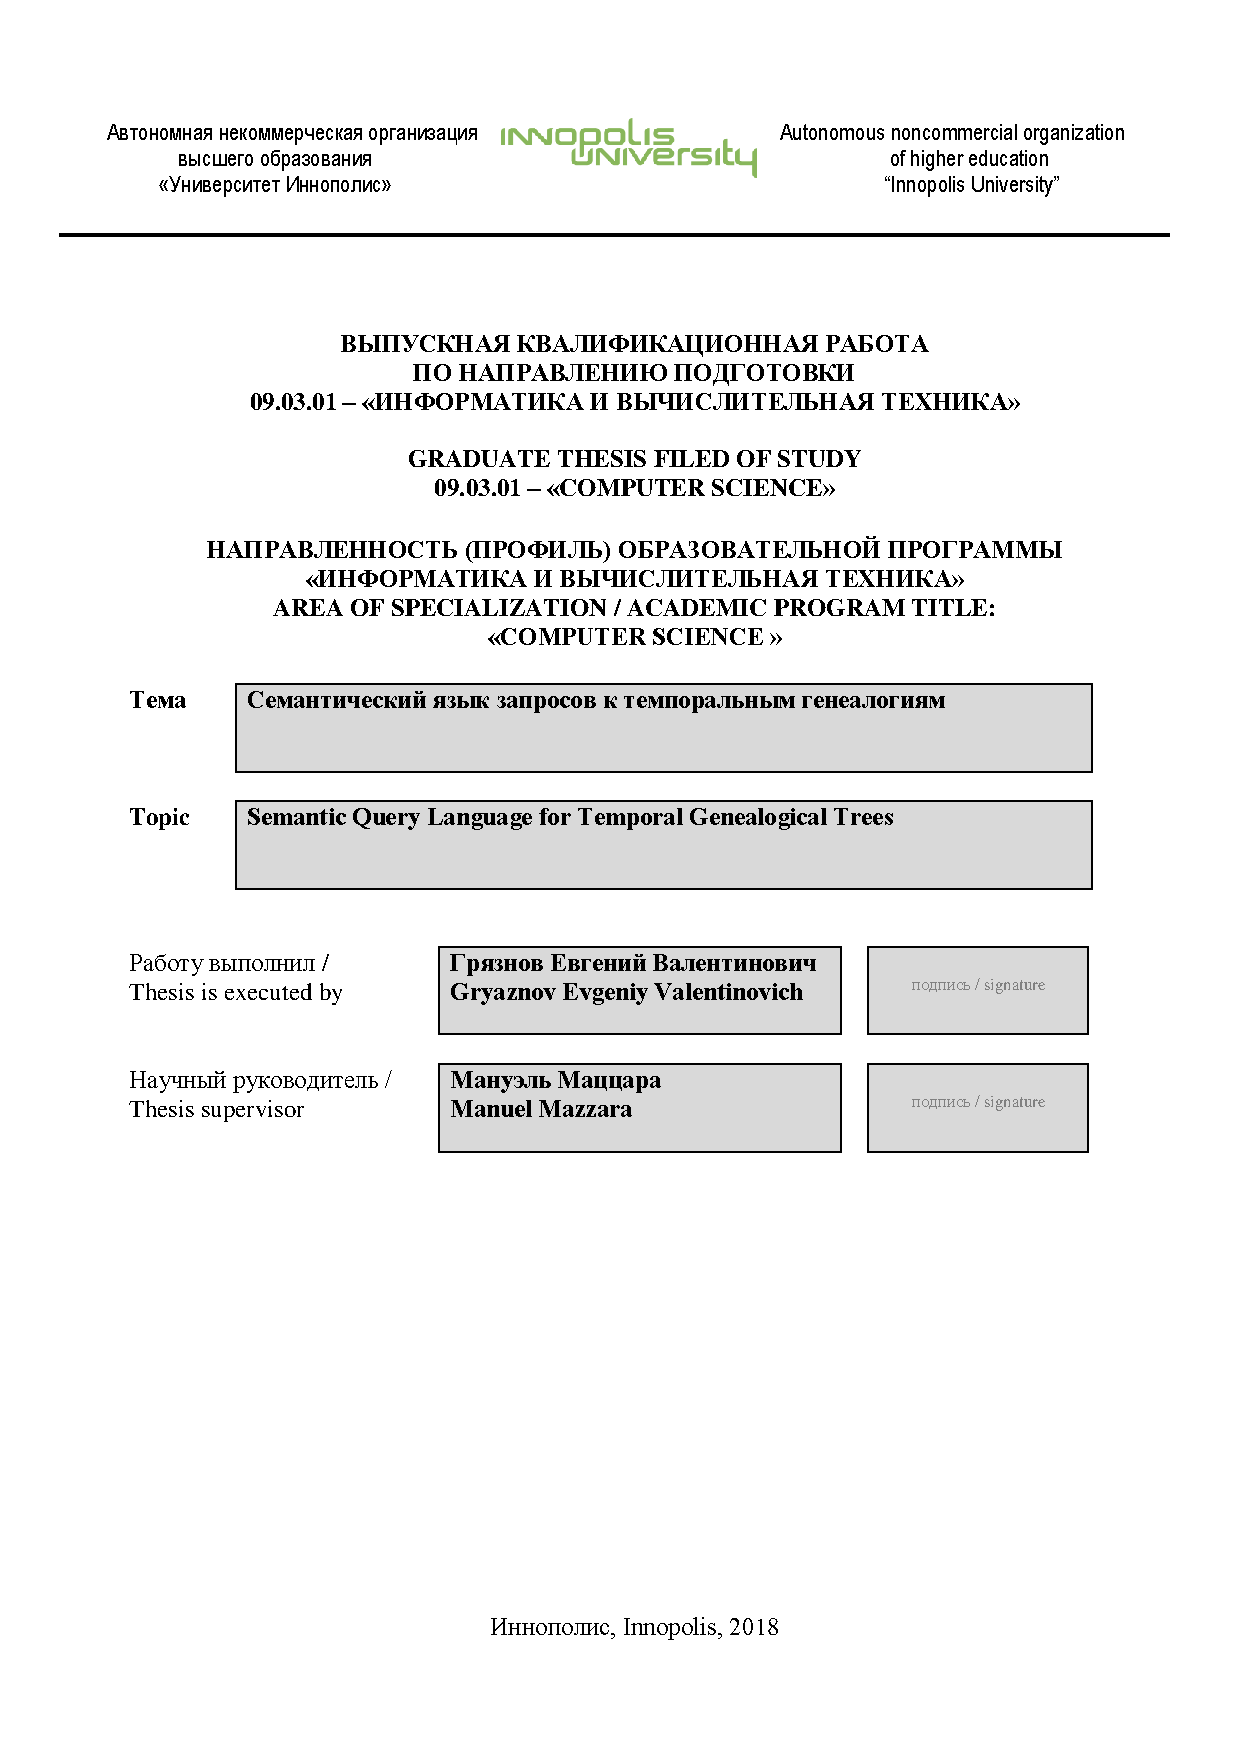
\includepdf[pages=-]{titles/BS.pdf}
\newpage
\thispagestyle{empty}

\mbox{}

\vspace{7cm}

\begin{flushright}

\textbf{\LARGE SEMANTIC QUERY LANGUAGE FOR TEMPORAL GENEALOGICAL TREES}

\vspace{0.1cm}

\rule{\linewidth}{0.15cm}%
\end{flushright}

\newpage
\dedication{To my parents and close relatives. This work would not be possible without their help.}
\newpage
\newpage
\thispagestyle{empty}


\begin{titlepage}


\begin{flushleft}
{\Large \bf
Acknowledgements
}


\vspace{0.01cm}

\rule{\linewidth}{0.05cm}%

\end{flushleft}

{
We would like to express our gratitude to  professor Manuel Mazzara, who kindly agreed to be our academic supervisor, and whose
help and support were virtually invaluable during the course of our work.

Additional thanks go to professor Nikolay Shilov for his useful advices and examination of the original topic proposal.
}

\end{titlepage}

\setcounter{page}{5}

\newpage
\thispagestyle{empty}
\mbox{}
\newpage

\tableofcontents
% \listoftables
\listoffigures

\newpage
\begin{abstract}
<<<<<<< HEAD
% give context (why it's important
% in this thesis we...
% present features
% implementation
% future work

We, as human beings, were always interested in the history of our families. From the medieval times the subject of genealogy
began to gain prominence, and now its considered one of the most important areas of history. Today computers play a crucial role
in the modern ancestry management, they are used to collect, store, analyse, sort and display the genealogical data. However,
current applications do not take advantage of the structure of a kinship system, and therefore they are inaccessible for a typical
user.

In this thesis we propose a new domain-specific language, called KISP, based on a formalisation of the English's kinship
system, for accessing and querying traditional genealogical trees. We implement its interpreter together with an ancestry
visualizer and a virtual assistant that helps the user in genealogy management. KISP is a dynamically typed LISP-like programming
language with such features as kinship term reduction and temporal information expression.

Our solution provides the user with a coherent genealogical framework that allows for a natural navigation over any traditional
family tree.

In the future work we would like add support for other, non-English systems of kinship, extend KISP with new features and
make the virtual assistant more intelligent.
=======
>>>>>>> 879ec8c8d5982b1008d17da8b7104f2aec7196a3

\end{abstract}


%!TEX root = root.tex

\chapter{Introduction}
\label{chap:intro}
\chaptermark{Optional running chapter heading}

\section{Spacing \& Type}
\label{sec:section}

This is a section. This is a citation without brackets \citen{A}. and this is one with brackets \cite{A}. These are multiple citations: [\citen{A, B, C}]. Here's a reference to a subsection: \ref{sec:subsection}. The body of the text and abstract must be double-spaced except for footnotes or long quotations. Fonts such as Times Roman, Bookman, New Century Schoolbook, Garamond, Palatine, and Courier are acceptable and commonly found on most computers. The same type must be used throughout the body of the text. The font size must be 10 point or larger and footnotes\footnote{This is a footnote.} must be two sizes smaller than the text\footnote{This is another footnote.} but no smaller than eight points. Chapter, section, or other headings should be of a consistent font and size throughout the ETD, as should labels for illustrations, charts, and figures.  

\subsection{Creating a Subsection}
\label{sec:subsection}

\subsubsection{Creating a Subsubsection}

\paragraph{This is a heading level below subsubsection}

And this is a quote: 
%
\begin{quote}
\blindtext
\end{quote}

This is a table:
% currsize is not set in the long table environment, so we need to set it before we set it up.
\makeatletter
\let\@currsize\normalsize
\makeatother

% tabular environments are set to be single-spaced in the  thesis class,  but long tables do not use tabular
% to get around this, set the spacing to single spacing at the start of the long table environment, and set it back to double-spacing at the end of it

\begin{longtable}{cc}
\caption[This is the title I want to appear in the List of Tables]{This is a caption.} \label{tab:pfams} \\
\hline
A & B \\
\hline
\endfirsthead
\multicolumn{2}{@{}l}{\textbf{Table \thetable} \ldots continued} \\
\hline
A & B \\
\hline
\endhead
a1 & b1 \\
a2 & b2 \\
a3 & b3 \\
a4 & b4 \\
\hline
\end{longtable}


The package ``upgreek'' allows us to use non-italicized lower-case greek letters. See for yourself: $\upbeta$, $\bm\upbeta$, $\beta$, $\bm\beta$. Next is a numbered equation:
\begin{align}
\label{eq:name}
\|\bm{X}\|_{2,1}={\underbrace{\sum_{j=1}^nf_j(\bm{X})}_{\text{convex}}}=\sum_{j=1}^n\|\bm{X}_{.,j}\|_2
\end{align}
The reference to equation (\ref{eq:name}) is clickable. 

\section[Theorems, Corollaries, Lemmas, Proofs, Remarks, Definitions\\ and Examples]{Theorems, Corollaries, Lemmas,\\ Proofs, Remarks, Definitions,\\ and Examples}

\begin{theorem}
\label{thm:onlytheorem}
\blindtext
\end{theorem}

\begin{proof}
I'm a (very short) proof.
\end{proof}

\begin{lemma}
I'm a lemma.
\end{lemma}

\begin{corollary}
I include a reference to Thm. \ref{thm:onlytheorem}.
\end{corollary}

\begin{proposition}
I'm a proposition.
\end{proposition}

\begin{remark}
I'm a remark. 
\end{remark}

\begin{definition}
I'm a definition. I'm a definition. I'm a definition. I'm a definition. I'm a definition. I'm a definition. I'm a definition. I'm a definition. I'm a definition. I'm a definition. I'm a definition. 
\end{definition}

\begin{example}
I'm an example.
\end{example}


\section[Optional table of contents heading]{Section with\\ linebreaks in\\the
name}


\Blindtext[2]





\chapter{Literature Review}
\label{chap:lr}
\chaptermark{Second Chapter Heading}
The purpose of this chapter is to give a brief survey of academic literature with respect to our thesis.
There are two major areas of Computer Science that are related to out research: Knowledge Representation (KR) and Natural Language
Processing (NLP). We will examine them one by one and highlight some of the most important works.

\section{Knowledge Representation}
The field of Knowledge Representation is concerned with how the knowledge about our physical world can be stored, managed and
utilized by computers. KR owes its existence to the more general field of Artificial Intelligence, which prompted the study of
encoding information about the physical reality into an intelligent system in such a way that it can be used by that system to
solve complex problems.

The main presupposition of the whole field of KR is that, in order for an intelligent agent to resolve a difficult problem, it
needs an access to some form of a knowledge specific to a particular domain and that knowledge should be stored inside the agent.
This presupposition is now widely known as the \textit{Knowledge Representation Hypothesis}:
\begin{quote}
    Any mechanically embodied intelligent process will be comprised of structural ingredients that (a) we as external observers
    naturally take to represent a propositional account of the knowledge that the overall process exhibits (b) independent of such
    external semantical attribution, play a formal but causal and essential role in engendering the behavior that manifests that
    knowledge.
\end{quote}
This original formulation of the hypothesis is due to Smith \cite{smithyp}.

Brachman and Levesque outlined the hypothesis in their article \textit{Expressiveness and tractability in Knowledge Representation
and Reasoning}\cite{krhyp}. The authors argue that the trade-off between \textit{expressiveness} of a knowledge-based system and
its \textit{tractability} (i.e. the ability to reason correctly) is intrinsic to every such system, and can only be partially
solved.  According to them, it's impossible to implement a knowledge-based system that will be both highly expressive and
completely tractable.

Moreover, the whole enterprise of encoding knowledge directly into an agent is proven to be useful only in domain-specific
applications, such as the famous \textit{block world} \cite{shrdlu} domain. A solution with at least partially hard-coded
knowledge is tremendously difficult to scale. Since the dawn of Machine Learning, the plausibility of the hypothesis is
continuously challenged. Indeed, it is questionable whether we can say about a neural network that it stores knowledge in the
weights of its neurons. Thus, today the field of KR doesn't enjoy that much popularity because the main focus of the AI community
has shifted to other areas, such as Deep Learning.

The most prominent advances in the KR field were the development of Description (Terminological) and Temporal logics and the
formulation of the concept of Ontology. They all are of great importance to our research, so we will survey them one by one.

\subsection{Ontologies}
The word "ontology", derived from the Greek word meaning "the study of being", was unwarrantably borrowed by computer scientists
from the namesake branch of philosophy concerned with the nature of reality. Despite being a useful coinage in
informatics, not all philosophers are content with such state of affairs \cite{confusion}.

The term "ontology" in Computer Science refers to the mechanism by which reality is compartmentalized into a strictly-defined
categories only to be read by machines later. According to Josephson et al. \cite{ontowhy} an ontology comprises a body of
knowledge about a particular domain of interest. However, we must distinguish between an abstract conceptualization of a
particular domain and a concrete instantiation of it. The latter is usually implied when the plural word "ontologies" is used.

The typical ontology consists of:
\begin{enumerate}
    \item{A finite set of \textit{concepts} (a.k.a. nodes, classes). Represents entities of a domain.}
    \item{A finite set of \textit{properties} (a.k.a. attributes, slots, roles). Represents what can be asked of a concept.}
    \item{A finite set of \textit{relationships} between concepts.}
    \item{A finite set of logical \textit{constraints}, which put the boundaries around what can and cannot be stored in an
        ontology.}
\end{enumerate}
At the first sight, the description of an ontology highly resembles that of a database. Indeed, it is true that every database can
be seen as a special case of an ontology, but not vise-versa. As noted in \cite{krhyp}, the power of ontologies lies not in what can
be said in them, but exactly \textit{what can be left unsaid}. For example, suppose we want to store the birth date of our
grandfather, but all we know about him is that he won a medal fighting in WWII.
Then we are forced, using a database, to left the \texttt{birth\_date} field empty, thus loosing the knowledge of his heroic deed.
But, we can eloquently express this knowledge in some ontological lisp-like language as:
\begin{verbatim}
    (set birth_date (father (father me)) (during WWI))
\end{verbatim}
Later we can use this fact to reason about our ancestor more efficiently.

Ontologies find their natural application in the context of our thesis.
Since the original formulation of a concept, a lot of software has been developed to manage ontologies, including such systems as
Protege, In4j and others. These systems have already been heavily used in the variety of different fields.

For instance, Tan Mee Ting \cite{tanfamily} designed and
implemented a genealogical ontology using Protege and evaluated its consistency with Pellet, HermiT and FACT++ reasoners. He
showed that it is possible to construct a family ontology using \textit{Semantic Web} \cite{web} technologies with full capability of
exchanging family history among all interested parties.

An ontology can be used to model any kind of family tree, but the problem arises when a user wants to query his relatives using
kinship terms. No standard out-of-the-box ontology query language is able to articulate statements such as in our example above.
Although an ontology can be tailored to do so, it is not in any way a trivial matter. Maarten Marx \cite{xcpath} addressed
this issue, but in the different area. He designed an extension for XPath, the first order node-selecting language for XML.

Catherine Lai and Steven Bird \cite{ling} described the domain of linguistic trees and discussed the expressive requirements for a
query language. Then they presented a language that can express a wide range of queries over these trees, and showed that the
language is first order complete. This language is also an extension of XPath.

Artale et al. \cite{artale} did a comprehensive survey of various temporal knowledge representation formalisms.
In particular, they analysed ontology and query languages based on the linear
temporal logic LTL, the multi-dimensional Halpern-Shoham interval temporal logic, as well as the metric temporal logic MTL. They
note that the W3C standard ontology languages, OWL 2 QL and OWL 2 EL, are designed to represent knowledge over a static domain,
and are not well-suited for temporal data.

\subsection{Temporal and Description Logics}
The usage of logic in the field of KR is motivated by its excellence in such areas as mathematics and computer science in general.
The early researches in KR saw the unharvested power of logic -- especially first-order logic -- as a main component in any
intelligent system. Subsequent works showed that FOL can provide semantics for specific kind of KR structures:
\textit{frames} \cite{frames}. Later, Brachman and Levesque proved \cite{krhyp} that we don't need the \textit{whole} FOL for that
purpose, but only certain fragments of it. Moreover, different fragments of FOL have different expressive power and tractability.
Thus, a research began under the label \textit{terminological systems}, only to be later renamed to
\textit{Description Logic} when the main focus was shifted to the properties of underlying logical systems.

Description Logic finds its application in the context of this thesis as a natural formalism for family trees. However, as
expressive as any DL can be, formulating the concept of time requires adding another modal operator. Any logic which handles time
is knows as \textit{temporal logic}. Philosophers have tried to put time into a coherent framework since Aristotle, in
the 20th century mathematicians and computer scientists proposed various formalisms, among which was Allens' \textit{interval
algebra}\cite{allen} and the temporal logic of Shoham\cite{shoh}. Thus, what we need in this thesis is an amalgamation of a
description and temporal logic.

The first successful attempt at integrating two logics is due to Schmiedel \cite{schmiedel}. He combined the DL in the tradition
of KL-ONE \cite{klone}, Shohams' \cite{shoh} temporal logic and Allens' \cite{allen} algebra into one unifying framework. The main
features of his formalism are the complete preservation of original DL and the use of lisp-like syntax for expressing roles,
concepts and time entires.

The application of temporal logic to graphs, relational databases and ontologies is also a heavily-invested subject.
Barcelo and Lubkin examined \cite{barcelo} several temporal logics over unranked trees and characterized commonly used fragments of
first-order (FO) and monadic second-order logic (MSO) for them. They also considered MSO sibling-invariant queries, that can use the
sibling ordering but do not depend on the particular one used, and captured them by a variant of the $\mu$-calculus with modulo
quantifiers.

Alexander Tuzhilin and James Clifford defined \cite{clif} a temporal algebra that is applicable to any temporal relational data
model supporting discrete linear bounded time. This algebra has the five basic relational algebra operators extended to the
temporal domain and an operator of linear recursion. They showed that this algebra has the expressive power of a safe temporal
calculus based on the predicate temporal logic with the "until" and "since" temporal operators.

Perry in his dissertation \cite{perry} highlighted that even in state-of-the-art ontological query languages, such as OWL,
expressing the concept of time is an arduous task. He augmented the \textit{Resource Description Framework} with temporal RDF
graphs and extended the W3C-recommended SPARQL query language to support these new structures.

An adequate representation of time is the holy grail among researchers in the field of ontology development.  Baratis et al.
\cite{toql} designed and implemented \textit{TOQL}: a high-level SQL-like language which is capable of expressing temporal
queries. They motivate the need for such a language by noting that conveying the concept of time using classical languages, such
as OWL, is proven to be difficult, although feasible. They also developed an application that supports translation and execution
of TOQL queries on temporal ontologies combined with a reasoning mechanism based on event calculus.

\section{Natural Language Processing}
The main goal of Natural Language Processing (NLP) field is to invent, study and implement algorithms and techniques that help a
computer understand an ordinary language, such as English, Russian, French or Swahili.

A lot of research in NLP is dedicated to the problem of querying a relational database in some natural language. Since the early
developments, a substantial progress has been achieved. For instance, Jeremy Ferrero et al. proposed and implemented \cite{fr2sql}
a solution to query any database, irrespective of its' schema, in virtually any natural language. They showed that it supports
more operations that most of the other translators. They tested their program on English and French languages.

Another similar attempt was made \cite{not} by Norouzifard et al. They implemented an expert system using Prolog to transform a
sentence in a natural language to SQL. Chaudhari \cite{chaudhari} presented a light weight technique of converting a natural
language statement into equivalent SQL
statement.

Nelken et al. took \cite{nelken} a step further and presented a novel controlled NL interface to \textit{temporal databases}, based on
translating NL questions into \textit{SQL/Temporal}, a temporal database query language. They noted that their translation method
is considerably simpler than previous attempts in this direction.

\section{Conclusions}
In this literature review we surveyed several major field in Computer Science. We showed that each of these fields has been advanced
considerably over the last half-century, especially the domain of ontologies. However, we did not find a research that would
satisfy all of the following criteria:
\begin{enumerate}
    \item{Employ either a temporal ontology or a temporal database to store knowledge of temporal family relations.}
    \item{Propose a solution for effective navigation in a genealogical tree via kinship terms.}
    \item{Design and implement a text parser for querying temporal ontologies in natural language.}
\end{enumerate}
Although there were articles that partially fulfill some of these requirements, none of them satisfied all.
This entails the novelty of our work.

\chapter{Methodology}
\label{chap:met}

\section{General Considerations}
\label{sec:general}
    The study of kin structures has its roots in the field of anthropology. Among the first foundational works was Henry Morgans'
    \textit{magnum opus} "Systems of Consanguity and Affinity of the Human Family"\cite{morgan}, in which he argues that all human
    societies share a basic set of principles for social organization along kinship\footnote{Recall that in this thesis, the word
    "kinship" includes relatives as well as in-laws} lines, based on the principles of \textbf{consanguinity}
    (kinship by blood) and \textbf{affinity} (kinship by marriage). At the same time, he presented a sophisticated schema of social evolution
    based upon the relationship terms, the categories of kinship, used by peoples around the world. Through his analysis of kinship
    terms, Morgan discerned that the structure of the family and social institutions develop and change according to a specific
    sequence. He was the first to recognize and record six kin structures that are present in numerous societies and cultures around
    the world.

    Bearing in mind the vast variety of possible options, we are going to settle on just one specific kin structure, which we shall
    call \textit{traditional kinship}. We will devote the entire chapter to describing and modelling this structure.

    Following Henry Morgan, we recognize two primary types of family bonds: marital (affinity) and
    parental (consanguinity). These bonds define nine basic kin terms: \textit{father, mother, son, daughter, husband, wife, parent,
    child and spouse}. Observe that combining them in different ways will yield all possible kinship terms that can and do exist.
    For instance, \textit{cousin} is \textit{a child of a child of a parent of a parent} of a particular person. Another example:
    \textit{mother-in-law} is just \textit{a mother of a spouse}.

    Let us introduce several useful definitions:
    \begin{definition}
        We call a kinship term \textbf{abstract} iff it can refer to relatives of different sex. For instance, the word
        "parent" is an abstract kinship term, because it refers to a mother as well as to a father. Other well known examples:
        \textit{cousin, spouse, sibling} and \textit{child}.
    \end{definition}

    \begin{definition}
        In contrast, a \textbf{concrete} kin term refers only to relatives of the same sex, e.g. \textit{brother, aunt} and
        \textit{nephew}.
    \end{definition}

    \begin{definition}
        A \textbf{dyadic} kin term express the relationship between individuals as they relate to one another symmetrically, e.g. if I
        am your cousin (sibling), then you are also my cousin (sibling). The few, and uncommon, English dyadic terms involve in-laws:
        \textit{co-mothers-in-law, co-fathers-in-law, co-brothers-in-law, co-sisters-in-law, co-grandmothers}, and
        \textit{co-grandfathers}.
    \end{definition}

    \begin{definition}
        An \textbf{ego} is a focal point of a genealogy, i.e. it is a person from whose point of view we will describe all other
        people using kin terms.
    \end{definition}

    Now Let us represent a traditional christian family tree as a special type of \textit{ontology} with its' own concepts,
    attributes, relations and constraints. Concepts are people in a family, their attributes are: \textit{name, birth date,
    birthplace, sex} and relations are parental and marital bonds with a wedding date.

    Together with the everything stated above, we have the following cultural constraints imposed on our genealogy:
    \begin{enumerate}
        \label{en:req}
        \item{Each person can have any finite number of children.}
        \item{Each person can have at most two parents of different sex.}
        \item{Each person can have at most one spouse of different sex.}
        \item{A spouse cannot be a \textit{direct relative}, i.e. a sibling or a parent. In other words, direct incest is
            prohibited.}
    \end{enumerate}

    When considering those prerequisites one should bear in mind that we deliberately focused only on rules, taboos and
    customs of one particular culture, namely American culture in the sense of Read \cite{read}. Under different assumptions and
    in further studies, these conditions can be relaxed and revisited.

    Apart from these four, here are two additional temporal constraints that express the interrelation between birth and wedding
    dates:
    \begin{enumerate}
        \item{No one can marry a person before he or she was born, i.e. a wedding date can only be strictly after a
            birth date of each spouse.}
        \item{A parent is born strictly before all of his (her) children.}
    \end{enumerate}
    Due to the general nature of these two constraints, they are always true in every genealogy and therefore can be safely
    assumed in our work.

    Every genealogy that meets these six requirements we shall call a \textbf{traditional family tree}. As the name "tree" suggests,
    we can indeed view this structure as a graph with its vertices as people and edges as bonds. Observe that every kinship term
    corresponds exactly to a \textit{path} between ego and specified relative. Under such a view, kin term becomes a set of instructions,
    telling how to get from the starting vertex \texttt{A} to the end vertex \texttt{B}. For example, consider the term
    \textit{mother-in-law}. What is it if not precisely a \textit{directive}: "firstly, go to my spouse, then proceed to her mother".
    The wonderful thing is that, due to the nature of kinship terminology, we can \textit{compose} them together to create
    new terms, even those which don't have their own name. This simple observation that we can see kinship terms as paths in a family
    tree underpins our entire thesis.

    Now, if we want to efficiently query a traditional family tree, we need to further investigate the mathematical features of
    the language of kinship terms. In the next sections we explore a formal model of kinship language, its syntax and semantics.
    Then we conclude this chapter with an examination of various approaches of tackling the concept of time. We also discuss
    possible augmentations to our model and the problem of \textit{term reduction}.

\section{Formal Language of Kinship}
\label{sec:formal}
    Here we present our attempt to model the language of traditional American, in the sense of Read\cite{read}, kinship terminology.
    There are three main characteristics that define every formal language: its syntax (spelling, how words are formed), semantics
    (what does particular word mean) and pragmatics (how a language is used). In order to describe it we must expound the first two.

    \subsection{Syntax}
    We use Backus-Naur Form to designate the syntax for our formal language. Let $\Sigma$ be the set of six basic kinship terms:
    \textit{father, mother, son, daughter, husband, wife}. Then we can express the grammar as follows:
    \begin{align*}
    \label{al:syntax}
    term ::= \Sigma | (term \cdot term) | (term \vee term) | (term)^{-1} | (term)^{\dagger}
    \end{align*}
    The first operation is called \textit{concatenation}, second -- \textit{fork}, third -- \textit{inverse} and the last --
    \textit{dual}. We denote this language by $\mathcal{L}$.

    Here are some examples of ordinary kinship terms expressed in our new language. Note that we deliberately omit superfluous
    parentheses and the composition sign for the sake of simplicity:
    \begin{itemize}
        \item{ Parent is $father \vee mother$. }
        \item{ Child is $son \vee daughter$. }
        \item{ Brother is $son (father \vee mother)$. }
        \item{ Sibling is $(son \vee daughter)(father \vee mother)$. }
        \item{ Uncle is $son(father \vee mother)(father \vee mother)$. }
        \item{ Daughter-in-law is $daughter \cdot husband$ }
        \item{ Co-mother-in-law is $mother(husband \vee wife)(son \vee daughter)$ }
    \end{itemize}
    From these examples you can see the real power of this language -- the power to express all possible used as well as not used
    kinship terms that can and do exist. Now the important step towards solving our main goal, developing a language for managing
    temporal genealogies, is to assign meaning to these words. From now on we distinguish between \textit{artificial} kinship terms,
    i.e. well-formed terms of our formalization, and \textit{natural} kin terms used in ordinary English. By referring to just terms,
    we mean the former, if nothing else is stated.

    \subsection{Semantics}
    Let $\Sigma^*$ stand for the set of all possible kin terms generated from the basis $\Sigma$ using the previously defined syntax.
    Let $\mathcal{G} = (V, E)$ be a traditional family tree with $V$ as a set of its vertices (people) and $E$ as a set of its
    edges (bonds). Moreover, because $\mathcal{G}$ is traditional, every person from the set $V$ have the following attributes:
    \begin{itemize}
        \item{A father. We will denote him as $father(p)$, a function that returns a \textit{set} containing at most one element.}
        \item{A mother. We will denote her by $mother(p)$.}
        \item{A set of his or her children: $children(p)$.}
        \item{A set of his or her sons: \[son(p) = \{c | c \in children(p) \land Male(p)\}\]}
        \item{A set of his or her daughters: \[daughter(p) = \{c | c \in children(p) \land Female(p)\}\]}
        \item{A spouse: $spouse(p)$.}
        \item{A husband: \[husband(p) = \{s | spouse(s) \land Male(p)\}\]}
        \item{A wife: \[wife(p) = \{s | spouse(s) \land Female(p)\}\]}
    \label{it:basic-func}
    \end{itemize}
    Due to the constraints stated in \ref{en:req}, result-set of $father$, $mother$, $spouse$, $husband$ and $wife$ can contain at
    most one element.

    Now we are ready to introduce \textbf{Denotational Semantics} for $\Sigma^*$. This name was chosen because it highly resembles
    namesake semantics of programming languages. Note that we regard kinship terms as \textit{functions} on subsets of $V$. Each
    function takes and returns a specific subset of all relatives, so its type is $f : \mathcal{P}(V) \to \mathcal{P}(V)$.

    We proceed by induction on the syntactic structure of $\mathcal{L}$. Let $t$ be an element of $\Sigma^*$, then:
    \begin{enumerate}
        \item{If $t \in \Sigma$, then $\llbracket t \rrbracket = F(t)$, where $F(t)$ assigns to each basic kin term its corresponding
            function from the list \ref{it:basic-func}.}
        \item{Term concatenation is a composition of two functions:
            \[\llbracket (t_1 \cdot t_2) \rrbracket = \llbracket t_1 \rrbracket \circ \llbracket t_2 \rrbracket\]}
        \item{Fork is a set-theoretic union of results of its sub-functions:
            \[\llbracket (t_1 \vee t_2) \rrbracket = p \mapsto \llbracket t_1 \rrbracket(p) \cup \llbracket t_2
        \rrbracket(p)\]}
        \item{Term inverse is exactly the inverse of its function:
            \[\llbracket t_1^{-1} \rrbracket = \llbracket t_1 \rrbracket^{-1}\]}
    \end{enumerate}
    The \textit{dual} operator ($\dagger$) is more difficult to define. We want it to mean exactly the same as the term, where the
    gender of each its basic sub-term is reversed, e.g. dual of "uncle" is "aunt", dual of "brother" is "sister" and so on.
    Here we can use induction once again:
    \begin{enumerate}
        \item{If $t \in \Sigma$, then $\llbracket t \rrbracket = D(t)$, where $D(t)$ is a basic term of opposite sex.}
        \item{Dual is distributive over concatenation, i.e. dual of concatenation is a concatenation of duals:
            \[\llbracket (t_1 \cdot t_2)^\dagger \rrbracket = \llbracket (t_1^\dagger \cdot t_1^\dagger) \rrbracket\]}
        \item{Dual is distributive over forking:
            \[\llbracket (t_1 \vee t_2)^\dagger \rrbracket = \llbracket (t_1^\dagger \vee t_2^\dagger ) \rrbracket\]}
        \item{Inverse commutes with dual:
                \[\llbracket (t^{-1})^{\dagger} \rrbracket = \llbracket (t^{\dagger})^{-1} \rrbracket\]}
    \end{enumerate}
    Observe that we also have the distributivity of concatenation over forking.
    This semantics allows us to efficiently navigate any family tree.

\section{Term Reduction}
\label{sec:reduc}
    Our artificial language has a problem: its too verbose. Indeed, to encode such ubiquitous kin terms as "uncle" or "great-nephew" one
    must use quite lengthy phrases that are hard to write and read. It is therefore important to have some sort of reduction mechanism
    for our language that will shorten long terms into a small set of common kinship relations to aid their understanding by a user.

    Firstly, let us analyse the problem. We have the following mapping $\omega$ between $\Sigma^*$ and the set of English kinship terms
    $\mathcal{W}$
    \begin{align*}
        son(father \vee mother) &\mapsto \text{brother}\\
        daughter(father \vee mother) &\mapsto \text{sister}\\
        father(father \vee mother) &\mapsto \text{grandfather}\\
        mother(father \vee mother) &\mapsto \text{grandmother}\\
        son(son \vee daughter) &\mapsto \text{grandson}\\
        \vdots\\
        father(son \vee daughter)(wife \vee husband)(son \vee daughter) &\mapsto \text{co-father-in-law}
    \end{align*}
    This dictionary allows us to effectively translate between kin terms of our artificial language $\mathcal{L}$ and their usual
    English equivalents. We can also view this mapping as a \textit{regular grammar} in the sense of Chomsky hierarchy\cite{chomsky}.
    However, note that we strictly prohibit mixing these two collections and therefore we deliberately avoid
    using words from the RHS in the LHS, because otherwise the grammar will lose its regularity and become \textit{at least}
    context-free, making the problem even more challenging. Let us define another function on top of $\omega$ that will replace the
    first sub-term $u \subset t$ in a term $t \in \Sigma^*$:
    \begin{align*}
        \Omega_u(t) = t[u / \omega(u)]
    \end{align*}
    Here the only change in meaning of $t[u / \omega(u)]$ is that the substitution takes place only once.

    Now the task can be stated thusly: given a term $t \in \Sigma^*$ find its shortest (in terms of the number of concatenations)
    translation under $\Omega$, i.e. which sub-terms need to be replaced and in what order.

    This problem can be easily reduced to that of of finding the desired point in the tree of all possible
    substitutions. Moreover, this point is actually a \textit{leaf}, because otherwise it is not the shortest one. But the latter
    can be solved by just searching for this leaf in-depth. Unfortunately, the search space grows exponentially with the
    number of entries in the dictionary $\omega$, thus making the naive brute-force approach unfeasible.

    Here we propose a heuristic greedy algorithm \ref{algo:red} that, although does not work for all cases, provides an expedient
    solution to the reduction problem in $O(n^2)$ time. Firstly, it finds the longest sub-term $u$ that exists in the dictionary
    $\omega$, then divides the term into two parts: left and right from $u$, after that it applies itself recursively to them, and
    finally it concatenates all three sub-terms together.

    Now let's analyse the time complexity of this algorithm:
    \begin{theorem}
        The execution time of the algorithm listed in \ref{algo:red} belongs to $\Theta(n^2)$.
    \end{theorem}
    \begin{proof}
        Let $T(n)$ be the execution time of the algorithm, where $n$ stands for the number of concatenations in a kin term.
        First of all, observe that $T(n)$ obeys the following recurrence:
        \begin{align}
            T(n) = 2 T(n / 2) + O(n^2)
        \end{align}
        Indeed, we make a recursive call exactly \textit{two} times and each call receives roughly the half of the specified term.
        During execution the function passes through two nested cycles, so one call costs us $O(n^2)$.

        Secondly, we use the \textbf{Master Method} from the famous book \textit{Introduction to Algorithms}\cite{cormen} by Cormen et al.
        In our case $a = 2$, $b = 2$, and $f(n) = O(n^2)$. Observe, that if we take $\epsilon$ to be any positive real number below
        one: $0 < \epsilon < 1$, then $f(n) = \Omega(n^{\log_ba + \epsilon}) = \Omega(n^{1 + \epsilon})$.

        Let us show that $f(n)$ satisfies the \textit{regularity} criterion: $af(n / b) \leqslant cf(n)$ for some constant $c < 1$.
        Indeed, just pick $c = 1/2$:
        \begin{align*}
            2f(n / 2) &\leqslant cf(n),\\
            2\frac{n^2}{4} &\leqslant cn^2,\\
            \frac{1}{2}n^2 &\leqslant cn^2,\\
            \frac{1}{2}n^2 &\leqslant \frac{1}{2}n^2
        \end{align*}
        Thus, we can use the third case from the Master Method, which tells us that $T(n) = \Theta(n^2)$.
    \end{proof}

    \subsection{Pursuing Confluence}
    Current approach listed in \ref{algo:red} has one major disadvantage: like any other greedy algorithm it can fail to choose a
    correct reduction path between two terms with equal amount of concatenations.
    We can alleviate this by augmenting our rewriting system, based on $\omega$ dictionary, with a feature called \textit{confluence},
    also known as \textit{Church-Rosser} property:
    \begin{definition}
        An abstract term rewriting system is said to possess \textbf{confluence}, if, when two terms $N$ and $P$ can be yielded from $M$,
        then they can be reduced to the single term $Q$. Figure \ref{fig:conf} depicts this scenario.
    \end{definition}
    Not only we can fix our reduction algorithm by introducing this property, but also we can improve the time complexity, making it
    linear.

    \begin{figure}
        \centering
        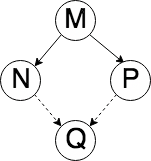
\includegraphics[width=0.2\linewidth]{figs/confluence.png}
        \caption{Confluence in a term rewriting system.}
        \label{fig:conf}
    \end{figure}

    One way to achieve confluence is to attach a single kinship term to any possible path in a family tree.
    Observe, that English kinship terms have a specific pattern that we can exploit. All relatives who are distant enough from ego
    have the following structure of their kin term:
    \begin{align*}
        n^{th} \text{ cousin } m^{th} \text{ times removed}
    \end{align*}
    In-laws also have their own pattern, where the ending "-in-law" is appended to a valid consanguine kinship term. However, this
    applies only to people, who are linked together by only one nuptial bond. For instance, there is no single term for a husband of
    ego's wife's sister. These relations can be accounted for by \textit{prefixing} "-in-law" with an ordinal, which shows the number
    of marital bonds that one should pass in order to go to such person. Under this representation, last example will receive the term
    "brother
    \textit{twice}-in-law". Generalizing that scheme we will get a pattern that looks like the following:
    \begin{align*}
        \langle \text{Consanguine kinship term} \rangle k^{th} \text{ times-in-law}
    \end{align*}

    We can also view this as an attribution of a distinct \textit{natural number} to every vertex with ego as an \textit{offset}, thus
    imposing a natural ordering on the set of all vertices. This assignment can be made in such a way that reducing a kinship term $n$
    will correspond \textit{exactly} to the calculation of $n$ from some arithmetic expression like $5 \cdot (2 + 3) + 4$, thus
    providing a \textbf{translation} between the language of all valid arithmetic expressions and our formal language of kinship
    $\mathcal{L}$.

    However, it is not the topic of this thesis, so we are leaving it to the considerations of future researches.

\section{Incorporating Time}
    Now the only matter that is left to address is an adequate representation of time. Historically, there are two main approaches
    for modelling time: point-based and interval-based. The former treats time as a single continuous line with distinguished points
    as specific \textit{events}, and the latter uses \textit{segments} of that line to represent time entries, which is more famous.
    For instance, it was used in Allen's interval algebra\cite{allen}. For the sake of simplicity we chose the former approach,
    because it can easily imitate intervals by treating them as endpoints of a line segment.

    Not only we want to talk about different events by modelling them as points on a line, but also we want to orient ourselves on
    that line, i.e. to know where we are, which events took place in the past and which will happen in the future. Thus, we need to
    select exactly one point that will stand for the present moment and call it "now". Then all point to the left will be in the past,
    and all point to the right will be in the future. Also, notice that any set with total ordering on it will suffice, because the
    continuous nature of a line is redundant in point-based model. Collecting everything together, we have the following formalisation
    of time:
    \begin{align*}
        \mathcal{M} = \langle T, now, \leqslant \rangle
    \end{align*}
    Where $T$ is a non-empty set with arbitrary elements, $now \in T$, and $\leqslant$ is a total ordering relation on $T$.

    Within this model we can reason about which event comes \textit{before} or \textit{after}, what events took place in the past or
    in the future, and so on.

    When considering family trees it's necessary to define only five predicates:
    \begin{enumerate}
        \item{$Before(x, y)$ is true iff $x < y$.}
        \item{$After(x, y)$ is true iff $x > y$.}
        \item{$During(x, s, f)$ is true iff $s \leqslant x \leqslant f$.}
        \item{$Past(x)$ is true iff $Before(x, now)$.}
        \item{$Future(x)$ is true iff $After(x, now)$.}
    \end{enumerate}
    Those relations are the basis from which all other operations on $\mathcal{M}$ can be defined. It is also interesting to note
    that, since any ordering relation generates a \textit{topology} over its structure, we can speak about time in terms of its
    topological properties.

    This observation concludes our methodology chapter.

\chapter{Implementation}
\label{chap:impl}
This chapter is dedicated to report the implementation of our genealogy management program.
Firstly, we present a specification for our new programming language named \textbf{KISP}:
\textbf{K}inship LI\textbf{SP}. Secondly, we describe the overall structure of the program, including its three major components:
Database Manager, Virtual Assistant and KISP Interpreter.

\section{KISP Language Specification}
\subsection{Grammar and Lexical Structure}
    Since KISP is a dialect of LISP, it inherits some syntax from the predecessor, but generally it is a new programming language. The
    grammar is presented with the help of Bacus-Naur notational technique. For the sake of simplicity we omit angle brackets and
    embolden non-terminal words. A plus, a star sign in a superscript and a question mark have the same meaning as in regular
    expressions.
    \begin{align*}
        \text{\textbf{term}} &::= \text{\textbf{literal}} | \text{\textbf{lambda}} | \text{\textbf{define}} | \text{\textbf{atom}} |
            (\text{\textbf{term}}^+) \\
        \text{\textbf{lambda}} &::= (\text{lambda (\textbf{reference}}^*\text{) \textbf{term}}) \\
        \text{\textbf{define}} &::= ( \text{define \textbf{reference} \textbf{term}}) \\
        \text{\textbf{reference}} &::= \text{\textbf{word}\{-\textbf{word}\}'?'?} \\
        \text{\textbf{word}} &::= \text{\textbf{letter}}^+ \\
        \text{\textbf{letter}} &::= a | b | ... | z | A | B | ... | Z \\
        \text{\textbf{atom}} &::= * | + | \text{concat} | \text{list} | \text{append} | ... \\
        \text{\textbf{literal}} &::= \text{void} | \text{true} | \text{false} | \text{people} | \text{vacant} | \text{now} |
            \text{\textbf{numeral}} | \text{\textbf{string}} \\
        \text{\textbf{numeral}} &::= \text{-?\textbf{digit}}^* \\
        \text{\textbf{digit}} &::= 0 | 1 | ... | 9 \\
        \text{\textbf{string}} &::= `\text{\textbf{symbol}}^*` \\
        \text{\textbf{symbol}} &::= \text{\textit{any non-blank ASCII symbol}}
    \label{al:bnf}
    \end{align*}
    As we can see from the definition, there are three kinds of terminals in the grammar: literals, references and atom functions,
    which are called simply \textbf{atom}s. Literals are instances of primitive types, such as \textit{Numeral}, \textit{String} or
    \textit{Boolean}, or special keywords. They stands for the following: "void" represents NULL type, "people" -- a list of
    all persons in a family tree, "now" -- the current time entry and "vacant" -- an empty list. References are used as definientia in
    "define" terms and as names for parameters in lambda terms. It is possible for a reference to end in a question mark, which means
    that it denotes an instance of \textit{Boolean} type. References can we written in so-called \textit{dash case}, so "long-name"
    and "very-long-name" are both legal. The only exception are names which start with the dash like "-illegal", they are invalid.

    Note that we allow niladic lambdas, so, for instance, this is a valid expression: \texttt{(lambda () 'Hello, World!')}. But at the
    same time \texttt{()} is not a well-formed term. We also prohibit "define" terms inside other terms, so this would not work:
    \texttt{(+ 2 (define three 3))}. Strings are nested in single quotes, integers, in KISP we call them "numerals", can start with a
    zero and be prefixed by a negative sign.

    Here is the complete list of all keywords in KISP: \textbf{true}, \textbf{false}, \textbf{define}, \textbf{lambda},
    \textbf{people}, \textbf{now}, \textbf{void}, \textbf{if}, \textbf{vacant}. The rule is that you can use as a reference everything
    you want as long as it is not a keyword, so you cannot redefine their standard behaviour, thus a programmer is unable to tamper
    with inner workings of the interpreter.

    As in all other dialects of LISP, a term \texttt{(f a b c ...)} means the \textit{execution} of a function $f$ with the
    specified arguments $f(a, b, c, ...)$. Of course, we can construct and call the higher-order functions as usual:
    \texttt{((twice square) 2)} will yield $16$, or \texttt{((compose inc inc) 0)} which prints $2$.

    Recursion also works as in any other LISP-like language. For example, here is the function that computes the $n$-th term of
    the famous Fibonacci sequence:
    \begin{verbatim}
    (define fibonacci
        (lambda (n)
            (if (< n 2)
                1
                (+ (fibonacci (- n 1)) (fibonacci (- n 2)))
            )
        )
    )
    \end{verbatim}
    However, using a reference before its definition is prohibited. For instance, the following code won't execute:
    \begin{verbatim}
    (+ 1 two)
    (define two 2)
    \end{verbatim}
    The interpreted will fail to recognize "two" as a valid reference in the first term and therefore will print an error message.
    The same applies to references in "define" term: cyclic definitions are forbidden:
    \begin{verbatim}
    (define zero (prev one))
    (define one (succ zero))
    \end{verbatim}

\subsection{Data Types}
    There are eight data types in KISP, four primitive and four composite. Primitive types: \textit{Boolean}, \textit{Numeral},
    \textit{Void} and \textit{String}. Composite: \textit{Function}, \textit{List}, \textit{Person} and \textit{Date}. An instance of
    a primitive type can be obtained by a literal, whereas a composite object is created only through calling a corresponding
    \textit{constructor} function. For instance, to make a list of three numbers one should use the following term: \texttt{(list 0 1
    2)}. However, there are three pre-defined global constants of composite types: \textit{now}, \textit{vacant} and \textit{people}.

    KISP is a \textit{dynamically} typed program language, which meas that information about a type of an entity is present only at
    execution time. This approach has certain benefits over \textit{static} typing as well as some disadvantages.

    For each type there are corresponding atomic functions provided by default to work with that type. Here we will present the atomic
    functions only for the type \textit{Person}, since it is the main element that distinguish KISP from other dialects. For the full
    documentation of other functions one can refer to the Appendix C\ref{chap:doc}.

    In order to create an instance of the type \textit{Person}, one should write \texttt{(person 'full name')}. This function will
    look up and return a person with stated full name in a linked family tree, or "void" if there is no person with such name.
    This function also has the following form: \texttt{(person 'first name' 'last name')}. All arguments are case-insensitive.

    The function \texttt{kinship} provides a convenient way to ascertain how a person $p_1$ is related to the person $p_2$:
    \texttt{(kinship $p_1$ $p_2$)}. It returns a \textit{list} of basic kin terms as strings. The content of such
    list corresponds exactly to a composite kinship term describing the relation of $p_1$ and $p_2$ to each other. For example, let us
    assume that there are two persons in our family tree: Alice and Bob. Alice is a niece of Bob, so if we to evaluate the term
    \texttt{(kinship (person 'alice') (person 'bob'))} we would get a term which is equal to \texttt{(list 'daughter' 'parent' 'son')}.
    The result can also be empty, but only if two persons are not related at all, i.e. the family tree has multiple connected components.

    In order to reduce a long kinship term generated by the latter method, one can use \textit{shorten} function that accepts the list
    of basic kin terms and performs the reduction algorithm outlined in the listing \ref{algo:red}. Using the previous example, running
    \texttt{(shorten (kinship (person 'alice') (person 'bob')))} will yield to the list of exactly one element: "niece". This function
    can be of use when printing the result of \textit{kinship}.

    Another useful function which return a specified attribute of a person is \textit{attr}. Here is how we can get a persons
    birthday: \texttt{(attr person 'birthday')}. This term produces the date of birth of a \texttt{person} as an object of type
    \textit{Date}. The list of all attributes accepted by \textit{attr} can be found in the full documentation \ref{doc:attr}.

    Of course, there are unitary functions corresponding to the denotations of basic kin terms: \textit{mother}, \textit{father},
    \textit{spouse} and \textit{children}. Here is how we can get a \texttt{person}s paternal grand-mother: \texttt{(mother (father
    person))}. All those functions return a list of respective relatives/in-laws. This list can be empty iff there is no such relative
    present in a family tree.

    Another interesting function is \textit{gen-dist}, which calculates the \textit{generational distance} between two persons.
    The distance $d$ is defined as the number of the level of the second person \textit{relative} to the first, where the level of the
    second person is considered to be zero:
    \begin{itemize}
        \item{The distance is a symmetric function: $d(x, y) = d(y, x)$, for all $x$ and $y$.}
        \item{It is zero for every two individuals from the same generation, including the person himself: $d(x, x) = 0$.}
        \item{Father located on the previous level, so $d(x, father(x)) = -1$.}
        \item{On the other hand, child inhabits the next level, thus $d(child(x), x) = 1$, and so on.}
    \end{itemize}
    For $d$ the calculation process is to start with zero, then increment each time we descend one level and decrement every time we
    ascend a level.

    The last function in the repertoire of the \textit{Person} type is \textit{put-kinship}. It is used to append a new entry
    into the $\omega$ dictionary, thus enhancing the capabilities of \textit{shorten}. For example, with \texttt{(put-kinship
    'son,parent,parent' 'uncle')} we can reduce avuncular terms. To correctly specify the formal kinship term, one must follow strict
    guidelines:
    \begin{enumerate}
        \item{Use only nine basic kinship terms.}
        \item{Separate them with a single comma without any in-between spaces.}
    \end{enumerate}

\section{Program Structure}
    % User requirements!!!
    % Если что спросят про bonds, просто сказать что в требованиях такого функционала не было.
    Firstly, we shall determine the user requirements for our program. Since there was no individual customer, who would say what
    features are indispensable and what are superfluous, we had to play this role ourselves. That eliminated the potential problems
    which one can encounter when trying to understand the needs of the user. Also, by putting ourselves into the situation of a
    potential customer, who often has rather trivial knowledge of IT, we gained an understanding of his point of view, which will be
    particularly helpful to us later.

    After careful considerations, we arrived at the following list of requirements:
    \begin{enumerate}
        \item{A user must be able to see his carefully crafted family tree in a nice visualisation.}
        \item{A user wants to move and scale this visualisation.}
        \item{A user must have an ability to move the nodes of his family tree.}
        \item{A user wants to add and remove members of his family.}
        \item{A user must be able to link his relatives together with nuptial and parental bonds.}
        \item{A user must be able to edit the profile of a person in his genealogy.}
        \item{A user must have an ability to manage many genealogies without losing his work.}
        \item{A user wants to ask and to get answers to meaningful questions about his family tree.}
    \end{enumerate}
    These eight items can be compartmentalized into three distinct categories: \textit{genealogy managing}, \textit{query answering}
    and \textit{family tree visualisation}. They form the basis for the components of our program. Observe, that if we apply a
    software design pattern known as \textit{Model-View-Controller}, we can merge the first and the third category into a single
    component, we will call it \textit{Genealogy Manager}, which will be responsible for displaying, handling and working with multiple
    genealogies, thus successfully covering all but one requirement from the list.

    Now, let's focus on the last requirement. Here the situation is different: in order to tackle it we need not to merge, but to
    split the second category, because of its challenging nature. If a user wants to ask questions, he firstly needs to
    \textit{formulate} them in some language that a machine can understand, which means that this language will be virtually
    inaccessible to a non-specialist. Therefore, it is of utmost importance to assist a user in expressing his questions.
    For that we propose the following solution: create a simple bot, whose set of English questions that it can answer will be rich
    enough to satisfy a users need for inquiries. Let's call such bot a \textit{Virtual Assistant}.
    Since we already have a formal language, we only need to develop its interpreter. Thus, we have two components that will cover the
    eighth requirement: a \textit{KISP Interpreter} and a Virtual Assistant.

    The figure \ref{fig:struct} depicts the general structure of our project. Notice how components are linked to each other and
    how some of them are encapsulated in others. From \ref{fig:struct} we can see that a user can interact only with
    \textit{Assistant} and \textit{Genealogy View} components, everything else is hidden from his sight. This is generally
    acknowledged to be the best approach to design user interfaces -- reducing degrees of freedom -- not only in software, but in
    all areas of technology.

    In the following sections we present the structure of the three software components that we identified.

\subsection{Genealogy Manager}
    As we can see from the figure \ref{fig:struct}, Genealogy Manager consists of three modules: Visualiser, Model and Database.
    The purpose of the first is to show a user nice and interactive view of his family tree. The second manages kinship
    records stored in DB and provides its interface for the rest of the application.

    Let's have a look at the third module: the Database, which stores the ontological \textit{axioms} of a family tree, that is, all
    persons and
    their connections to each other in the form of table records. We chose a relational database for that purpose and not our own
    solution mainly because the current ones are much more efficient and because it was too costly to enrich KISP with such
    features. We selected SQLite as the RDBMS engine for our application, since it is compact and effective at the same time.

    The Entity-Relation diagram\ref{fig:er} has been converted to tables in the following way:
    \begin{enumerate}
        \item{The main entity \textit{Person} is presented as a table incorporating all information about people in a family tree. It
            has ID field as a primary key. }
        \item{The $1-1$ relation "wed" encodes the marital bonds between people, and $1-N$ relation "beget" encodes the parental
            bonds. They both are represented as separate tables, which contain the edges of a family tree. The former is also made to
            be symmetrical, i.e. $wed(x, y) \iff wed(y, x)$, which allows for more coherent reasoning about genealogy. Symmetry means that
            each record in the table 'wed' is doubled and reversed after being inserted.}
    \end{enumerate}
    Each row is loaded from DB and stored in the next sub-component, \textit{Model}, as a graph data structure. The model defines all
    the necessary methods to work with this graph, including \textit{Breadth-First Search} algorithm that is used to find to minimal
    path between two vertices.

    The \textit{Visualiser} then renders this tree inside a predefined rectangular region, which can be further scaled and moved by
    the special camera class. This class implements a lightweight version of a 2D graphical engine.

    \subsection{Virtual Assistant}
    After careful considerations, we settled on a list of English questions that our virtual assistant, named \textit{Ami}, can answer.
    This list is rich enough to satisfy any user and, at the same time, short enough to allow an actual implementation.
    Observe, that the list actually defines a \textit{infinite} amount of potential questions by including special
    \texttt{<reference>} part, which we define by again using convenient Bacus-Naur notation:
    \begin{align*}
        \text{\textbf{reference}} &::= \text{\textbf{name}} | \text{my \textbf{relative}} |
        \text{my \textbf{relative}s' \textbf{relative}} | \text{\textbf{relative} of \textbf{reference}} | \text{I} | \text{me} |
        \text{myself} \\
        \text{\textbf{relative}} &::= \text{\textbf{basic}} | \text{uncle} | \text{brother} | ... \\
        \text{\textbf{basic}} &::= \text{parents} | \text{parent} | \text{son} | ...
    \end{align*}
    Where \textbf{relative} stands for an \textit{image} of the dictionary $\omega$, \textbf{name} for the full name of a person and
    \textbf{basic} for all primal kinship terms.

    \begin{enumerate}
        \item{How is \texttt{<reference>} related to \texttt{<reference>}?}
        \item{How am I related to \texttt{<reference>}?}
        \item{Who is \texttt{<reference>}?}
        \item{Who is (a or an) \texttt{<relative>} of \texttt{<reference>}?}
        \item{Where \texttt{<reference>} (was or were) born?}
    \end{enumerate}
    As we can see, questions in this list have a coherent and static structure that can be parsed by machine, thus allowing us to take
    the most straightforward approach and implement them directly hard-coded string constants.

    Besides questions, Ami also accepts KISP queries that it channels to the Interpreter. For example, in order to query
    all females in genealogy one need to send the following message to Ami:
    \begin{verbatim}
    (filter (lambda (p) (= 'FEMALE' (attr p 'sex'))) people)
    \end{verbatim}
    Due to the incredibly versatile nature of our programming language, we can confidently say that there is no ineffable queries.
    Therefore, a user can always express himself at least in KISP, if not in English.

    Secondly, Ami can perform various auxiliary commands, such as:
    \begin{enumerate}
        \item{'Show [me] \texttt{<reference>}.' This command will center the view of a family tree on the specific person that is
            mentioned in the \texttt{<reference>}. If there are many persons, Ami will choose the first one. It is useful when we want
            to quickly locate a particular relative in a big tree.}
        \item{'Load filename.lisp', this command reads the specified file and executes its content as KISP source code. It may be of
            use when we need to quickly introduce new functions and definitions.}
    \end{enumerate}

    Finally, we must note that Ami is a \textit{context-free} assistant, which means that it takes into account only the very last
    message of the user. However, there is an important exception to this rule: if a user sends a message for the first time
    referring to himself, Ami will ask who he is, because there is no such information available by default. Context awareness of the
    virtual assistant is an interesting topic for future research, as well as considering different channels of user input, such as
    voice recognition.

    \subsection{KISP Interpreter}
    For the implementation of the KISP language we chose the most straightforward approach: firstly parse the source code, secondly,
    construct an AST, then perform an evaluation of that tree starting from its leaves, and finally output the result of the
    evaluation. However, in order to expedite this process, we introduced a caching mechanism, which remembers what terms yields to
    what results. Term caching is a questionable feature, because in some cases it may produce incorrect results. Bugs may arise when
    we redefine some term that has been cached previously.

    For example, let's evaluate the following terms:
    \begin{verbatim}
        (define ego (person 'John Doe'))

        (= ego ego)

        (define ego (person 'Joe Sixpack'))

        (= 'Joe' (attr ego 'first name'))
    \end{verbatim}
    The last term will be incorrectly evaluated to \texttt{false}, since the result of the term \texttt{ego} was not updated in the
    cache table. To alleviate that problem we added the command \texttt{flush} into our virtual assistant, which removes all entries
    from that table.

    This concludes the implementation chapter.

\chapter{Evaluation and Discussion}
\label{chap:eval}

\ldots

\chapter{Conclusion}
\label{chap:conclusion}
% какая была проблема
% значимость
% как мы её решили
% с какими трудностями столкнулись
% что ещё можно сделать
In this work we solved the problem of efficient navigation in temporal genealogies by designing domain-specific programming language
KISP and implementing its interpreter. To further facilitate the use of our program, tree visualiser and virtual assistant have
been developed. By the term "efficient" we mean three things:
\begin{enumerate}
    \item{It should have high expressive power.}
    \item{It must be fast enough.}
    \item{It should be as intuitive as possible.}
\end{enumerate}
We are certain that our project fully covers every one of them.

From the very start of our history, we gathered, analysed and composed information about our ancestors and relatives.
Although, with the ubiquitous use of computers, we can do it more effectively than ever, the present market solutions are
found to be inadequate in one way or the other. Particularly, the vast majority of them are either lacking expressiveness or are
too complicated and, therefore, require a special training just to be used. In contrast, our project manages to be a user-friendly
application, while at the same time having a high level of expressive power.

During the course of our work we faced such challenges as reducing long kinship terms and developing a swift 2D graphical
engine, all of which were successfully solved.

\section{Future Work}
However, there are some topics yet left to tackle in the area of kinship and genealogy management. On the theoretical side, there
is a problem of total term reduction and formal language enrichment. It is also interesting to shift attention to other languages
and cultures with different kinship structures, such as Russian or Hawaiian. The constructed formalism can be considered from the
algebraical side, focusing on its many mathematical properties as a special type of an algebraic system.

On the practical side, one can consider to improve the virtual assistant component. Besides already mentioned Voice Generation \&
Recognition technology, it can be made context-aware, which will increase its intelligence. Additionally, the family ontology can
be enhanced to incorporate information about divorces and deaths. The performance of the interpreter can be significantly improved
by introducing \textit{Just-in-Time} compilation.

Further improvements may also include new data types and standard functions for KISP language. Specifically, it is beneficial to
add a \texttt{char} type that represents individual characters in a string. Another useful feature is support for \textit{variadic
lambdas} and \textit{closures}, which will significantly increase the versatility of KISP.

Moreover, one can also consider including capabilities for a logical reasoning into KISP. They will be applicable for inferring
implicit time constraints for events, whose exact date is unknown. For instance, if we are uninformed about a birthday of a
person, but we do know his parents and his children birthdays, we can justifiably bound this missing date to a specific time
interval.


%% REFERENCES
\bibliographystyle{IEEEtran}
\bibliography{thesis}
\appendix
\chapter{Pseudocode Listings}
\begin{algorithm}[caption={Kinship Term Reduction}, label={algo:red}]
    input: kinship term $t$.
    note: $\omega$ is a dictionary of kinship terms.
    note: Functions "leftPart(t, u)" and "rightPart(t, u)" return the sub-term of $t$
    note: from the left of sub-term $u$ or from the right respectively.
    note: Function "subterm(t, i, j)" returns the
    note: sub-term of the kinship term $t$ between indices $i$ and $j$.
    output: reduced kin term.
    function shorten(t)
    begin
        maxShortenableSubterm $\gets$ empty
        currentSubterm $\gets$ empty
        for i $\gets$ 0 to length(t) do
        begin
            for j $gets$ length(t) - i to 0 do
            begin
                currentSubterm $\gets$ subterm(t, i, j)
                if length(currentSubterm) $>$ length(maxShortenableSubterm)
                    and $\omega$(currentSubterm) is not empty
                then
                    maxShortenableSubterm = currentSubterm
            end
        end
        return shorten(leftPart(t, maxShortenableSubterm))
               $\cdot$ $\omega(maxShortenableSubterm)$
               $\cdot$ shorten(rightPart(t, maxShortenableSubterm))
    end
\end{algorithm}

\chapter{Figures}

\begin{figure}
    \centering
    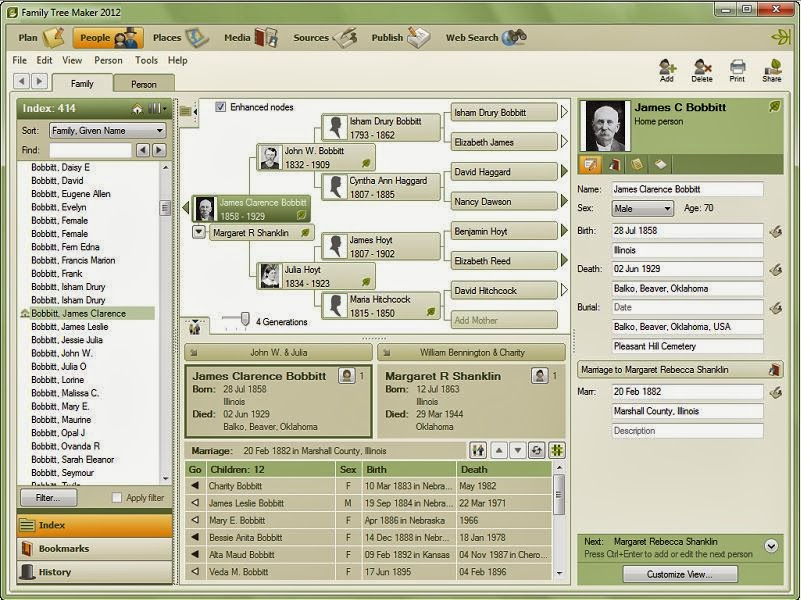
\includegraphics[width=\linewidth]{figs/ftmShot.png}
    \caption{Main Screen of Family Tree Maker}
    \label{fig:ftmShot}
\end{figure}

\begin{figure}
    \centering
    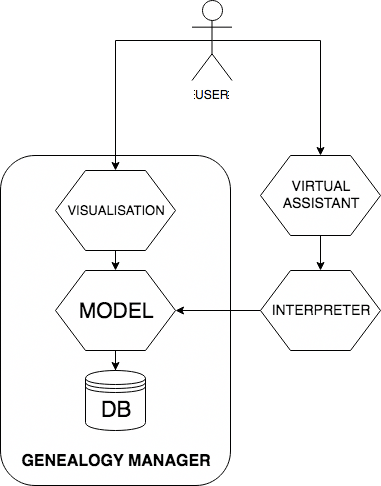
\includegraphics[width=\linewidth]{figs/structure.png}
    \caption{Structure of System Components}
    \label{fig:struct}
\end{figure}

\chapter{Documentation of Standard KISP Functions}
\label{chap:doc}
Note that two commas after a parameter name is a signature means any positive number of arguments. Also, a backtick (\texttt{`})
denotes a single quote (').

\subsection{void}
\begin{itemize}
    \item Name: Void Constant
    \item Signature: \texttt{void}
    \item Description: A unique constant of type Void.
    \item Examples :
        \begin{itemize}
            \item \texttt{(= void void) = true}
            \item \texttt{(= void 3) = false}
        \end{itemize}
    \item Type : \[Void\]
\end{itemize}

\subsection{define}
\begin{itemize}
    \item Name: Define
    \item Signature: \texttt{(define reference term)}
    \item Description: Creates an abbreviation \texttt{reference} for the specified lisp \texttt{term}.
    \item Arguments:
        \begin{itemize}
            \item \textbf{reference} : A shortcut for \texttt{term}. Can only be composed of lowercase English letters and a dash.
            \item \textbf{term} : A well-formed lisp term as a designatum. Keep in mind that you can use \texttt{reference} in \texttt{term} to create recursion, but make sure that there are no cyclic definitions.
        \end{itemize}
    \item Examples :
        \begin{itemize}
            \item \texttt{(define name 'John Doe')}
            \item \texttt{(define two 2)}
            \item \texttt{(define twice (lambda (n) (f (f n))))}
        \end{itemize}
    \item Type : \[Void\]
    \item Notes : This function cannot be used inside another functions, only as a top-level term. You cannot redefine standard keywords like define itself, \texttt{lambda} and so on.
\end{itemize}

\subsection{lambda}
\begin{itemize}
    \item Name: Lambda
    \item Signature: \texttt{(lambda (args) lambda-term)}
    \item Description: Instantiates a new anonymous function which takes its arguments \texttt{args} and applies them to the \texttt{term}
    \item Arguments:
        \begin{itemize}
            \item \textbf{args} : A list of argument names for this lambda-term separated by space
            \item \textbf{term} : A well-formed lisp term that will be applied to arguments \texttt{args}
        \end{itemize}
    \item Examples :
        \begin{itemize}
            \item \texttt{(lambda () 2)}
            \item \texttt{(lambda (n) (* 2 n)}
            \item \texttt{(lambda (a, b) (+ a (* a b))}
        \end{itemize}
    \item Notes : You can use only English letters and dashes for names of the arguments. Argument list is separated by single space. Empty argument list is permitted
\end{itemize}

\subsection{and}
\begin{itemize}
    \item Name: And
    \item Signature: \texttt{(and boolean..)}
    \item Description: Performs a logical AND operation on N boolean terms
    \item Arguments:
        \begin{itemize}
            \item \textbf{boolean1} : First boolean conjunct
            \item \textbf{boolean2} : Second boolean conjunct
            \item \textbf{...} : ...
            \item \textbf{booleanN} : N-th boolean conjunct
        \end{itemize}
    \item Examples :
        \begin{itemize}
            \item \texttt{(and true) = true}
            \item \texttt{(and false true) = false}
            \item \texttt{(and true true false) = false}
        \end{itemize}
    \item Type : \[(Boolean)^n  o Boolean\]
    \item Notes : All conjuncts will be evaluated, always. Function accepts any non-zero number of arguments.
\end{itemize}

\subsection{or}
\begin{itemize}
    \item Name: Or
    \item Signature: \texttt{Performs a logical OR operation on N boolean terms.}
    \item Description: (or boolean..)
    \item Arguments:
        \begin{itemize}
            \item \textbf{boolean1} : First boolean disjunct
            \item \textbf{boolean2} : Second boolean disjunct
            \item \textbf{booleanN} : N-th boolean disjunct
        \end{itemize}
    \item Examples :
        \begin{itemize}
            \item \texttt{(or true) = true}
            \item \texttt{(or false true) = true}
            \item \texttt{(or false false true) = true}
        \end{itemize}
    \item Type : \[(Boolean)^n \to Boolean\]
    \item Notes : All disjuncts will be evaluated, always. Function accepts any non-zero number of arguments.
\end{itemize}

\subsection{not}
\begin{itemize}
    \item Name: Not
    \item Signature: \texttt{(not boolean-term)}
    \item Description: Performs a logical NOT operation on exactly one boolean term.
    \item Arguments:
        \begin{itemize}
            \item \textbf{boolean} : A boolean term, whose value will be inverted.
        \end{itemize}
    \item Examples :
        \begin{itemize}
            \item \texttt{(not true) = false}
            \item \texttt{(not false) = true}
        \end{itemize}
    \item Type : \[Boolean \to Boolean\]
    \item Notes : This function accepts only one boolean argument.
\end{itemize}

\subsection{during}
\begin{itemize}
    \item Name: During
    \item Signature: \texttt{(during date-point date-star date-end)}
    \item Description: Checks whether the date \texttt{date-point} is after \texttt{date-start} and before \texttt{date-finish}. Returns \texttt{true} iff \texttt{date-point} belongs to the time interval [\texttt{date-start}, \texttt{date-date-end}]
    \item Arguments:
        \begin{itemize}
            \item \textbf{date-point} : A date which is going to be checked for belonging to the time interval [\texttt{date-start}, \texttt{date-end}]
            \item \textbf{date-start} : A starting point of the time interval
            \item \textbf{date-end} : An ending point of the time interval
        \end{itemize}
    \item Examples :
        \begin{itemize}
            \item \texttt{(during WWII 1900 2000) = true}
        \end{itemize}
    \item Type : \[(Date)^3 \to Boolean\]
    \item Notes :
\end{itemize}

\subsection{before}
\begin{itemize}
    \item Name: Before
    \item Signature: \texttt{(before date-pointA date-pointB)}
    \item Description: Checks whether date point A is happened before date point B. Returns true or false accordingly.
    \item Arguments:
        \begin{itemize}
            \item \textbf{date-pointA} : First time point, which is needed to be before the second point for the formula to result in \texttt{true}.
            \item \textbf{date-pointB} : Second time point
        \end{itemize}
    \item Examples :
        \begin{itemize}
            \item \texttt{(before WWII WWI) = false}
        \end{itemize}
    \item Type : \[(Date)^2 \to Boolean\]
    \item Notes :
\end{itemize}

\subsection{after}
\begin{itemize}
    \item Name: After
    \item Signature: \texttt{(after date-pointA date-pointB)}
    \item Description: Checks whether date point A is happened after date point B. Returns true or false accordingly.
    \item Arguments:
        \begin{itemize}
            \item \textbf{date-pointA} : First time point, which is needed to be after the second point for the formula to result in \texttt{true}.
            \item \textbf{date-pointB} : Second time point
        \end{itemize}
    \item Examples :
        \begin{itemize}
            \item \texttt{(after WWII WWI) = false}
        \end{itemize}
    \item Type : \[(Date)^2 \to Boolean\]
    \item Notes :
\end{itemize}

\subsection{date}
\begin{itemize}
    \item Name: Date
    \item Signature: \texttt{(date string-date)}
    \item Description: Parses \texttt{string-date} and returns a date object created from this string
    \item Arguments:
        \begin{itemize}
            \item \textbf{string-date} : A string representation of a date object. Should be in the format: dd.mm.year.
        \end{itemize}
    \item Examples :
        \begin{itemize}
            \item \texttt{(date '10.11.1995')}
            \item \texttt{(date '01.01.1900')}
        \end{itemize}
    \item Type : \[String \to Date\]
    \item Notes : You should strictly follow the date format in order for this function to work. Void is returned iff invalid string is passed to this function.
\end{itemize}

\subsection{list}
\begin{itemize}
    \item Name: List
    \item Signature: \texttt{(list args..)}
    \item Description: Creates a list object from passed arguments.
    \item Arguments:
        \begin{itemize}
            \item \textbf{args} : A space-separated list of objects out of which list will be created
        \end{itemize}
    \item Examples :
        \begin{itemize}
            \item \texttt{(list 1 2 3 4)}
            \item \texttt{(list 'first' 'second' 'third')}
            \item \texttt{(list 1 'two' (date '1.1.1990'))}
        \end{itemize}
    \item Type : \[(Object)^n \to List\]
    \item Notes : Accepts non-zero number of arguments. Parameters are allowed to be of different type. If you want an empty list, use the term \texttt{vacant}.
\end{itemize}

\subsection{join}
\begin{itemize}
    \item Name: Join
    \item Signature: \texttt{(join list..)}
    \item Description: Concatenates N lists
    \item Arguments:
        \begin{itemize}
            \item \textbf{list} : A space-separated sequence of lists to be concatenated
        \end{itemize}
    \item Examples :
        \begin{itemize}
            \item \texttt{(join list1 list2)}
            \item \texttt{(join list)}
            \item \texttt{(join (list 1 2) (list 3) (list 4)) = [1, 2, 3, 4]}
        \end{itemize}
    \item Type : \[(List)^n \to List\]
    \item Notes : Accepts non-zero number of arguments.
\end{itemize}

\subsection{count}
\begin{itemize}
    \item Name: Count
    \item Signature: \texttt{(count list)}
    \item Description: Returns the number of elements in \texttt{list}.
    \item Arguments:
        \begin{itemize}
            \item \textbf{list} : A list object.
        \end{itemize}
    \item Examples :
        \begin{itemize}
            \item \texttt{(count (list 1 2 3)) = 3}
            \item \texttt{(count (list 1)) = 1}
        \end{itemize}
    \item Type : \[List \to Numeral\]
    \item Notes : Accepts a non-zero number of arguments.
\end{itemize}

\subsection{filter}
\begin{itemize}
    \item Name: Filter
    \item Signature: \texttt{(filter predicate list)}
    \item Description: Takes a predicate together with a list and retains only those elements, which satisfy predicates' condition.
    \item Arguments:
        \begin{itemize}
            \item \textbf{predicate} : Lambda function of type $Object \to Boolean$, which we apply to all elements in \texttt{list}
            \item \textbf{list} : A list which needs to be filtered
        \end{itemize}
    \item Examples :
        \begin{itemize}
            \item \texttt{(filter odd? (list 1 2 3 4 5)) = [1, 3, 5]}
            \item \texttt{(filter uppercase? (list 'TEST' 'test' 'tEsT')) = ['TEST']}
        \end{itemize}
    \item Type : \[(Lambda \times List) \to List\]
\end{itemize}

\subsection{at}
\begin{itemize}
    \item Name: At
    \item Signature: \texttt{(at list index)}
    \item Description: Returns the \texttt{index}-th element of \texttt{list}.
    \item Arguments:
        \begin{itemize}
            \item \textbf{list index} : A list whose element at specified place will be taken
        \end{itemize}
    \item Examples :
        \begin{itemize}
            \item \texttt{(at (list 1 2 3 4) 3) = 4}
            \item \texttt{(at (list 0 1 2) 3) = void}
            \item \texttt{(at (list 0 1 2 3 4 5) -1) = 5}
        \end{itemize}
    \item Type : \[(List \times Numeral) \to Object\]
    \item Notes : Indices start with 0. If there is no item at specified index, than Void is returned. Indices can be negative, e.g. -1 points to last element, -2 -- penultimate, -3 -- antepenultimate and so on.
\end{itemize}

\subsection{append}
\begin{itemize}
    \item Name: Append
    \item Signature: \texttt{(append list item..)}
    \item Description: Includes all \texttt{item}s in the end of \texttt{list}.
    \item Arguments:
        \begin{itemize}
            \item \textbf{list} : A list to which items will be included
            \item \textbf{item..} : A space-separated sequence of objects that will be included in the \texttt{list}
        \end{itemize}
    \item Examples :
        \begin{itemize}
            \item \texttt{(append list 1)}
            \item \texttt{(append (list 1 2 3) 4 5 6) = [1, 2, 3, 4, 5, 6]}
        \end{itemize}
    \item Type : \[(List \times (Object)^n) \to List\]
    \item Notes : You can pass any positive number of arguments
\end{itemize}

\subsection{mod}
\begin{itemize}
    \item Name: Modulo
    \item Signature: \texttt{(mod a n)}
    \item Description: Computes a residue modulo \texttt{n}, i.e. the remainder of a natural division of \texttt{a} by \texttt{n}
    \item Arguments:
        \begin{itemize}
            \item \textbf{a} : Dividend
            \item \textbf{n} : Divisor
        \end{itemize}
    \item Examples :
        \begin{itemize}
            \item \texttt{(mod 5 2) = 1}
            \item \texttt{(mod 10 4) = 2}
        \end{itemize}
    \item Type : \[(Numeral)^2 \to Numeral\]
    \item Notes : Divisor should not be zero.
\end{itemize}

\subsection{add}
\begin{itemize}
    \item Name: Addition, or $+$
    \item Signature: \texttt{(+ number..)}
    \item Description: Calculates sum of all \texttt{number}s.
    \item Arguments:
        \begin{itemize}
            \item \textbf{number..} : A non-empty space-separated sequence of numeral terms.
        \end{itemize}
    \item Examples :
        \begin{itemize}
            \item \texttt{(+ 2) = 2}
            \item \texttt{(+ 1357 10) = 1367}
            \item \texttt{(+ 1 2 3) = 6}
        \end{itemize}
    \item Type : \[(Numeral)^n \to Numeral\]
    \item Notes : The function accepts any positive number of arguments
\end{itemize}

\subsection{mul}
\begin{itemize}
    \item Name: Multiplication, or $*$
    \item Signature: \texttt{(* number..)}
    \item Description: Calculates product of all \texttt{number}s.
    \item Arguments:
        \begin{itemize}
            \item \textbf{number..} : A non-empty space-separated sequence of numeral terms.
        \end{itemize}
    \item Examples :
        \begin{itemize}
            \item \texttt{(* 2) = 2}
            \item \texttt{(* 1357 10) = 13570}
            \item \texttt{(* 1 2 3) = 6}
        \end{itemize}
    \item Type : \[(Numeral)^n \to Numeral\]
    \item Notes : The function accepts any positive number of arguments
\end{itemize}

\subsection{lessEqual}
\begin{itemize}
    \item Name: Less Or Equal, $<=$
    \item Signature: \texttt{(<= a b)}
    \item Description: Checks whether \texttt{a} <= \texttt{b}
    \item Arguments:
        \begin{itemize}
            \item \textbf{a} : first numeral to be compared
            \item \textbf{b} : second numeral to be compared
        \end{itemize}
    \item Examples :
        \begin{itemize}
            \item \texttt{(<= 2 5) = true}
            \item \texttt{(<= 10 3) = false}
        \end{itemize}
    \item Type : \[(Numeral)^2 \to Boolean\]
    \item Notes : Function expects exactly two numerals as arguments.
\end{itemize}

\subsection{less}
\begin{itemize}
    \item Name: Less, or just $<$
    \item Signature: \texttt{(< a b)}
    \item Description: Checks whether $a < b$
    \item Arguments:
        \begin{itemize}
            \item \textbf{a} : first numeral to be compared
            \item \textbf{b} : second numeral to be compared
        \end{itemize}
    \item Examples :
        \begin{itemize}
            \item \texttt{(< 2 5) = true}
            \item \texttt{(< 10 3) = false}
        \end{itemize}
    \item Type : \[(Numeral)^2 \to Boolean\]
    \item Notes : Function expects exactly two numerals as arguments.
\end{itemize}

\subsection{greater}
\begin{itemize}
    \item Name: Greater, or just $>$
    \item Signature: \texttt{(> a b)}
    \item Description: Checks whether $a > b$
    \item Arguments:
        \begin{itemize}
            \item \textbf{a} : first numeral to be compared
            \item \textbf{b} : second numeral to be compared
        \end{itemize}
    \item Examples :
        \begin{itemize}
            \item \texttt{(> 5 2) = true}
            \item \texttt{(> 10 13) = false}
        \end{itemize}
    \item Type : \[(Numeral)^2 \to Boolean\]
    \item Notes : Function expects exactly two numerals as arguments.
\end{itemize}

\subsection{greaterOrEqual}
\begin{itemize}
    \item Name: Greater Or Equal, $>=$
    \item Signature: \texttt{(>= a b)}
    \item Description: Checks whether $a \ge b$
    \item Arguments:
        \begin{itemize}
            \item \textbf{a} : first numeral to be compared
            \item \textbf{b} : second numeral to be compared
        \end{itemize}
    \item Examples :
        \begin{itemize}
            \item \texttt{(>= 5 5) = true}
            \item \texttt{(>= 3 5) = false}
        \end{itemize}
    \item Type : \[(Numeral)^2 \to Boolean\]
    \item Notes : Function expects exactly two numerals as arguments.
\end{itemize}

\subsection{concat}
\begin{itemize}
    \item Name: String Concatenation
    \item Signature: \texttt{(concat string..)}
    \item Description: Concatenates all \texttt{string}s
    \item Arguments:
        \begin{itemize}
            \item \textbf{string} : A non-empty space-separated sequence of string objects.
        \end{itemize}
    \item Examples :
        \begin{itemize}
            \item \texttt{(concat 'test' 'ing' ' concat') = 'testing concat'}
            \item \texttt{(concat 'hello ' 'world!') = 'hello world!'}
        \end{itemize}
    \item Type : \[(String)^n \to String\]
    \item Notes : This function accepts any positive number of arguments.
\end{itemize}

\subsection{of-type?}
\begin{itemize}
    \item Name: Of Type?
    \item Signature: \texttt{(of-type? o type)}
    \item Description: Returns true iff object \texttt{o} has a \texttt{type}.
    \item Arguments:
        \begin{itemize}
            \item \textbf{o type} : An object whose type needs to be checked
            \item \textbf{type} : A name of a type
        \end{itemize}
    \item Examples :
        \begin{itemize}
            \item \texttt{(of-type? 'test' 'string) = true}
            \item \texttt{(of-type? 3 'date') = false}
        \end{itemize}
    \item Type : \[(Object \times String) \to Boolean\]
    \item Notes : The name of a type should be entered precisely
\end{itemize}

\subsection{equals}
\begin{itemize}
    \item Name: Equals, or $=$
    \item Signature: \texttt{(= objA objB)}
    \item Description: Returns true iff \texttt{objA} and \texttt{objB} are exactly the same thing.
    \item Arguments:
        \begin{itemize}
            \item \textbf{objA} : First object to be compared
            \item \textbf{objB} : Second object to be compared
        \end{itemize}
    \item Examples :
        \begin{itemize}
            \item \texttt{(= '3' 3) = false}
            \item \texttt{(= 10 10) = true}
            \item \texttt{(= (date '1.1.1999') (date '1.1.1999')) = true}
        \end{itemize}
    \item Type : \[(Object)^2 \to Boolean\]
    \item Notes : Function accepts exactly two arguments
\end{itemize}

\subsection{sub}
\begin{itemize}
    \item Name: Subtraction, or $-$
    \item Signature: \texttt{(sub m s)}
    \item Description: Calculates the difference between m (minuend) and s (subtrahend).
    \item Arguments:
        \begin{itemize}
            \item \textbf{m} : Minuend
            \item \textbf{s} : Subtrahend
        \end{itemize}
    \item Examples :
        \begin{itemize}
            \item \texttt{(sub 5 2) = 3}
            \item \texttt{(sub 0 1) = -1}
        \end{itemize}
    \item Type : \[(Numeral)^2 \to Numeral\]
    \item Notes : Accepts exactly two arguments.
\end{itemize}

\subsection{div}
\begin{itemize}
    \item Name: Integer division
    \item Signature: \texttt{(div n m)}
    \item Description: Calculates the quotient from integer division of n (dividend) by m (divisor)
    \item Arguments:
        \begin{itemize}
            \item \textbf{n} : Dividend
            \item \textbf{m} : Divisor
        \end{itemize}
    \item Examples :
        \begin{itemize}
            \item \texttt{(div 10 2) = 5}
            \item \texttt{(div 5 2) = 2}
            \item \texttt{(div 3 2) = 1}
        \end{itemize}
    \item Type : \[(Numeral)^2 \to Numeral\]
    \item Notes : Accepts exactly two arguments. Divisor shouldn't be zero, or exception will be thrown
\end{itemize}

\subsection{father}
\begin{itemize}
    \item Name: Father
    \item Signature: \texttt{(father person)}
    \item Description: Returns father of the specified person
    \item Arguments:
        \begin{itemize}
            \item \textbf{person} : A link to a person object
        \end{itemize}
    \item Examples :
        \begin{itemize}
            \item \texttt{(father (person 'John' 'Golt'))}
            \item \texttt{(father (person 'Emma Clark'))}
        \end{itemize}
    \item Type : \[Person \to Person\]
    \item Notes : Accepts and returns exactly one object of type Person. If provided person doesn't have a father, returns empty
        list.
\end{itemize}

\subsection{mother}
\begin{itemize}
    \item Name: Mother
    \item Signature: \texttt{(mother person)}
    \item Description: Returns mother of the specified person
    \item Arguments:
        \begin{itemize}
            \item \textbf{person} : A link to a person object
        \end{itemize}
    \item Examples :
        \begin{itemize}
            \item \texttt{(mother (person 'John' 'Golt'))}
            \item \texttt{(mother (person 'Emma Clark'))}
        \end{itemize}
    \item Type : \[Person \to Person\]
    \item Notes : Accepts and returns exactly one object of type Person. If provided person doesn't have a mother, returns empty
        list.
\end{itemize}

\subsection{spouse}
\begin{itemize}
    \item Name: Spouse
    \item Signature: \texttt{(spouse person)}
    \item Description: Returns spouse of the specified person
    \item Arguments:
        \begin{itemize}
            \item \textbf{person} : A link to a person object
        \end{itemize}
    \item Examples :
        \begin{itemize}
            \item \texttt{(spouse (person 'John' 'Golt'))}
            \item \texttt{(spouse (person 'Emma Clark'))}
        \end{itemize}
    \item Type : \[Person \to Person\]
    \item Notes : Accepts and returns exactly one object of type Person. If provided person doesn't have a spouse, returns empty
        list.
\end{itemize}

\subsection{children}
\begin{itemize}
    \item Name: Children
    \item Signature: \texttt{(children person)}
    \item Description: Returns list of persons' children
    \item Arguments:
        \begin{itemize}
            \item \textbf{person} : A link to a person object
        \end{itemize}
    \item Examples :
        \begin{itemize}
            \item \texttt{(children (person 'John' 'Golt'))}
            \item \texttt{(children (person 'Emma Clark'))}
        \end{itemize}
    \item Type : \[Person \to List\]
    \item Notes : Returns empty list if the specified person is childless.
\end{itemize}

\subsection{gen-dist}
\begin{itemize}
    \item Name: Generation Distance
    \item Signature: \texttt{(gen-dist person1 person2)}
    \item Description: Calculates the \texttt{generation distance} between two people
    \item Arguments:
        \begin{itemize}
            \item \textbf{person1} : First person
            \item \textbf{person2} : Second person
        \end{itemize}
    \item Examples :
        \begin{itemize}
            \item \texttt{(gen-dist me (father me)) = -1}
            \item \texttt{(gen-dist me (grandfather me)) = -2}
            \item \texttt{(gen-dist me (son me)) = 1}
        \end{itemize}
    \item Type : \[(Person)^2 \to Numeral\]
    \item Notes : Generation distance is the difference between generations. The generation of the first person is assumed to be zero, and the generation of the second person is calculated accordingly.
\end{itemize}

\subsection{person}
\begin{itemize}
    \item Name: Person
    \item Signature: \texttt{(person first-name)}
    \item Description: Returns the person with specified first and last name
    \item Arguments:
        \begin{itemize}
            \item \textbf{first-name} : A string with the first name of a person
        \end{itemize}
    \item Examples :
        \begin{itemize}
            \item \texttt{(person 'John' 'Doe')}
        \end{itemize}
    \item Type : \[String^2 \to Person\]
    \item Notes : The function also accepts full name in one string: (person 'Full Name')
\end{itemize}

\subsection{kinship}
\begin{itemize}
    \item Name: Kinship
    \item Signature: \texttt{(kinship person1 person2)}
    \item Description: Returns a list of basic kinship terms (strings) that represents how is \texttt{person1} related to \texttt{person2}.
    \item Arguments:
        \begin{itemize}
            \item \textbf{person1 person2} : First person
        \end{itemize}
    \item Examples :
        \begin{itemize}
            \item \texttt{(kinship (father me) me) = ['father']}
            \item \texttt{(kinship (uncle me) me) = ['son','parent','parent']}
        \end{itemize}
    \item Type : \[Person^2 \to List\]
    \item Notes : Basic kinship terms are: \texttt{father}, \texttt{mother}, \texttt{parent}, \texttt{son}, \texttt{daughter}, \texttt{child}, \texttt{husband}, \texttt{wife}, \texttt{spouse}
\end{itemize}

\subsection{attr}
\label{doc:attr}
\begin{itemize}
    \item Name: Get Attribute
    \item Signature: \texttt{(attr person prop)}
    \item Description: Returns requested property \texttt{prop} of the specified \texttt{person}.
    \item Arguments:
        \begin{itemize}
            \item \textbf{person} : Person of interest
            \item \textbf{prop} : Property of interest
        \end{itemize}
    \item Examples :
        \begin{itemize}
            \item \texttt{(attr (person 'John Golt') 'first name') = 'John'}
            \item \texttt{(attr (person 'John Golt') 'sex') = 'MALE'))}
        \end{itemize}
    \item Type : \[(Person \times String) \to Object\]
    \item Notes : All possible properties are: \texttt{first name}, \texttt{last name}, \texttt{full name}, \texttt{second name},
        \texttt{birth}, \texttt{birth date}, \texttt{date of birth}, \texttt{gender}, \texttt{sex}, \texttt{birthplace}, \texttt{phone}, \texttt{phone number}, \texttt{tel}, \texttt{email}, \texttt{e-mail}, \texttt{wedding}.
\end{itemize}

\subsection{shorten}
\begin{itemize}
    \item Name: Shorten Kinship Term
    \item Signature: \texttt{(shorten list)}
    \item Description: Reduces the list of basic kinship terms.
    \item Arguments:
        \begin{itemize}
            \item \textbf{list} : List of basic kinship terms.
        \end{itemize}
    \item Examples :
        \begin{itemize}
            \item \texttt{(shorten (kinship person1 person2))}
        \end{itemize}
    \item Type : \[List \to List\]
    \item Notes :
\end{itemize}

\subsection{put-kinship-term}
\begin{itemize}
    \item Name: Put Kinship Term
    \item Signature: \texttt{(put-kinship-term list-basic shortcut)}
    \item Description: Registers a new custom kinship term \texttt{shortcut} from the list of basic terms \texttt{list-basic}. The new term can be used later in \texttt{shorten} function.
    \item Arguments:
        \begin{itemize}
            \item \textbf{list-basic} : Non-empty list of basic kinship terms
            \item \textbf{shortcut} : A string with a definition of a new kinship term
        \end{itemize}
    \item Examples :
        \begin{itemize}
            \item \texttt{(put-kinship-term (list 'son' 'parent' 'parent') 'uncle')}
            \item \texttt{(put-kinship-term (list 'son' 'parent') 'brother')}
        \end{itemize}
    \item Type : \[Void\]
    \item Notes :
\end{itemize}

\subsection{vacant}
\begin{itemize}
    \item Name: Vacant List
    \item Description: An empty list constant
    \item Examples :
        \begin{itemize}
            \item \texttt{(count vacant) = 0}
        \end{itemize}
    \item Type : \[List\]
\end{itemize}

\subsection{map}
\begin{itemize}
    \item Name: List Mapping Function
    \item Signature: \texttt{(map f list) or (map f l1 l2)}
    \item Description: Applies the unary function f to each element of a specified list or constructs a third list by applying binary f to each consecutive pair of elements from lists l1 and l2.
    \item Arguments:
        \begin{itemize}
            \item \textbf{f} : An unary or binary mapping function
            \item \textbf{list} : A list whose elements will be mapped one by one
            \item \textbf{l1} : A list, each item of which will be supplied to f as a first argument
            \item \textbf{l2} : A list, each item of which will be supplied to f as a second argument
        \end{itemize}
    \item Examples :
        \begin{itemize}
            \item \texttt{(map square (first-n 3)) = [1, 4, 9]}
            \item \texttt{(map + (list 1 2 3) (list 4 5 6)) = [5, 7, 9]}
        \end{itemize}
    \item Type : \[Either Lambda \times List \to List or Lambda \times (List)^2 \to List\]
    \item Notes :
\end{itemize}

\subsection{tail}
\begin{itemize}
    \item Name: Tail
    \item Signature: \texttt{(tail list)}
    \item Description: Return the tail, i.e. all but the first element of a list
    \item Arguments:
        \begin{itemize}
            \item \textbf{list} : A specified list
        \end{itemize}
    \item Examples :
        \begin{itemize}
            \item \texttt{(tail (list 0 1 2)) = (list 1 2)}
            \item \texttt{(tail (list 1)) = vacant}
        \end{itemize}
    \item Type : \[List \to List\]
    \item Notes : This function is analogous to \texttt{cdr} in Common Lisp.
\end{itemize}

\subsection{head}
\begin{itemize}
    \item Name: Head
    \item Signature: \texttt{(head list)}
    \item Description: Returns the head, i.e. the first element of a list
    \item Arguments:
        \begin{itemize}
            \item \textbf{list} : A specified list
        \end{itemize}
    \item Examples :
        \begin{itemize}
            \item \texttt{(head (list 1 2 3))= 1}
            \item \texttt{(head vacant) = void}
        \end{itemize}
    \item Type : \[List \to Object\]
    \item Notes : This function is analogous to \texttt{car} in Common Lisp.
\end{itemize}

\subsection{now}
\begin{itemize}
    \item Name: Now
    \item Signature: \texttt{now}
    \item Description: A date constant that hold the current time.
    \item Examples :
        \begin{itemize}
            \item \texttt{(before now now) = false}
        \end{itemize}
    \item Type : \[Date\]
\end{itemize}

\subsection{people}
\begin{itemize}
    \item Name: People
    \item Signature: \texttt{people}
    \item Description: A constant of type List that holds all persons in a family tree.
    \item Examples :
        \begin{itemize}
            \item \texttt{(head people)}
        \end{itemize}
    \item Type : \[List\]
\end{itemize}

\end{document}
